\section{Propuesta}

Este trabajo propone el \textit{Marco de Aprendizaje Inclusivo y Adaptativo}
(MAIA), una arquitectura de referencia para sistemas tutores inteligentes
orientados a las Aulas Integradas del MEP. El marco integra en un diseño
cohesivo tres componentes técnicos que la literatura ha desarrollado de
forma aislada: detección emocional multimodal, seguimiento cognitivo
automatizado mediante procesamiento del lenguaje natural, y un motor de
adaptación basado en aprendizaje por refuerzo con control docente en el
bucle (\textit{human-in-the-loop}).

% ------------------------------------------------------------
\subsection{Visión General de la Arquitectura}
% ------------------------------------------------------------

El MAIA se organiza en cuatro capas funcionales con responsabilidades
claramente delimitadas (Fig.~\ref{fig:arquitectura}). La \textbf{capa de
percepción} captura señales multimodales del estudiante (video, audio y
registro de interacción). La \textbf{capa de análisis} procesa en paralelo
el estado afectivo y el nivel cognitivo del estudiante a partir de esas
señales. La \textbf{capa de decisión} combina ambos resultados para
seleccionar la siguiente acción pedagógica, activando la intervención del
docente únicamente cuando la decisión supera un umbral de impacto
configurable. La \textbf{capa de presentación} entrega el contenido
adaptado al estudiante y provee al docente de un tablero de supervisión
con alertas.

\begin{figure}[htbp]
\centering
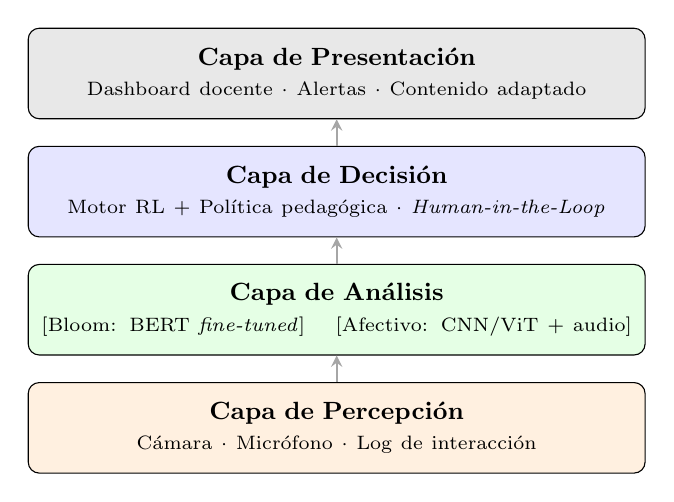
\begin{tikzpicture}[
    base/.style={draw=black, rounded corners=4pt,
                 text width=7.6cm, minimum height=1.15cm,
                 align=center, font=\small},
    arr/.style={->, >=stealth, thick, gray!70}
]
\node[base, fill=gray!18] (pres) at (0,4.5) {
    \textbf{Capa de Presentación}\\
    \scriptsize Dashboard docente $\cdot$ Alertas $\cdot$ Contenido adaptado
};
\node[base, fill=blue!10] (dec) at (0,3.0) {
    \textbf{Capa de Decisión}\\
    \scriptsize Motor RL + Política pedagógica $\cdot$ \textit{Human-in-the-Loop}
};
\node[base, fill=green!10] (anal) at (0,1.5) {
    \textbf{Capa de Análisis}\\
    \scriptsize {[Bloom: BERT \textit{fine-tuned}]} \quad {[Afectivo: CNN/ViT + audio]}
};
\node[base, fill=orange!12] (perc) at (0,0) {
    \textbf{Capa de Percepción}\\
    \scriptsize Cámara $\cdot$ Micrófono $\cdot$ Log de interacción
};
\draw[arr] (perc.north) -- (anal.south);
\draw[arr] (anal.north) -- (dec.south);
\draw[arr] (dec.north) -- (pres.south);
\end{tikzpicture}
\caption{Arquitectura de referencia del Marco de Aprendizaje Inclusivo y
Adaptativo (MAIA). Las flechas indican el flujo de información entre capas.}
\label{fig:arquitectura}
\end{figure}

Las cuatro capas de la figura describen el flujo de información a alto nivel;
los módulos que se detallan a continuación son las unidades de implementación
que realizan ese flujo. El \textbf{Módulo de Percepción Afectiva} abarca tanto la capa de percepción
como la rama afectiva de la capa de análisis, ya que
el procesamiento emocional es inseparable de la adquisición de la señal. El
\textbf{Módulo de Seguimiento Cognitivo} corresponde a la rama cognitiva de
la capa de análisis. El \textbf{Motor de Adaptación} implementa la capa de
decisión, y la \textbf{Interfaz Docente} materializa la capa de presentación.

% ------------------------------------------------------------
\subsection{Módulo de Percepción Afectiva}
% ------------------------------------------------------------

El módulo de percepción afectiva captura y fusiona tres flujos de señales
del estudiante para producir un vector de estado emocional
$\mathbf{e} \in [0,1]^{n}$ actualizado en tiempo real. La \textbf{rama
visual} emplea una red convolucional (CNN) o un transformer de visión (ViT)
que procesa los fotogramas de la cámara web y clasifica micro-expresiones
faciales en categorías como frustración, aburrimiento, atención o
entusiasmo. La \textbf{rama de audio} realiza análisis prosódico sobre la
señal del micrófono ---velocidad de habla, tono, duración de las pausas---
para obtener una señal complementaria del estado emocional que no depende
de la expresión facial. La \textbf{rama de interacción} extrae patrones
implícitos del comportamiento del estudiante sobre la interfaz: latencia de
respuesta, frecuencia de errores y velocidad de navegación entre pantallas.

Las tres ramas se combinan mediante \textit{fusión tardía} (\textit{late
fusion}): cada rama produce su propia estimación de estado emocional de
forma independiente, y un componente de fusión pondera y agrega los
resultados. Esta estrategia permite que cada rama sea entrenada, actualizada
o reemplazada de forma independiente sin afectar al resto del módulo, lo
que resulta especialmente importante en un contexto de despliegue progresivo
como el del MEP, donde la disponibilidad de hardware puede variar entre
instituciones.

% ------------------------------------------------------------
\subsection{Módulo de Seguimiento Cognitivo}
% ------------------------------------------------------------

El módulo de seguimiento cognitivo evalúa el nivel de complejidad cognitiva
de las interacciones del estudiante y lo mapea a uno de los seis niveles de
la Taxonomía de Bloom: recordar, comprender, aplicar, analizar, evaluar y
crear. La entrada del módulo son las respuestas textuales del estudiante ---ya
sea texto escrito o transcripción de audio--- y su salida es un par
$(b,\, p)$, donde $b \in \{1,\ldots,6\}$ es el nivel de Bloom inferido y
$p \in [0,1]$ es la confianza asociada.

El mecanismo de clasificación se basa en un modelo BERT ajustado finamente
(\textit{fine-tuned}) sobre un corpus de ítems de evaluación etiquetados
con niveles de Bloom, siguiendo la metodología de Das et al.~\cite{Das2020},
que alcanzó un 89\,\% de precisión en clasificación multiclase. Para el
contexto costarricense, el modelo se re-entrenaría sobre material curricular
del MEP en español, alineando las categorías de Bloom con los indicadores de
logro oficiales. Cada respuesta del estudiante actualiza el modelo del
estudiante en tiempo real: si $p$ supera un umbral mínimo de confianza, $b$
se registra en el historial cognitivo de la sesión; de lo contrario, el
sistema solicita una actividad de clarificación antes de actualizar el
estado.

% ------------------------------------------------------------
\subsection{Motor de Adaptación}
% ------------------------------------------------------------

El motor de adaptación toma como entrada el vector emocional $\mathbf{e}$,
el nivel cognitivo $b$ y el historial de la sesión, y produce la siguiente
acción pedagógica $a^{*}$ del espacio de acciones disponibles: avanzar al
siguiente nivel de Bloom, reforzar el nivel actual con un ejercicio
alternativo, cambiar la modalidad de presentación del contenido, o pausar y
notificar al docente.

El motor combina una política inicial basada en reglas pedagógicas del MEP
con un algoritmo de aprendizaje por refuerzo que refina dicha política con
cada interacción. La política inicial codifica criterios curriculares
concretos: no avanzar al siguiente nivel de Bloom si la confianza del
clasificador es inferior a un umbral predefinido, o pausar la actividad si
el vector emocional indica frustración sostenida durante más de $k$ turnos
consecutivos. Este mecanismo de arranque resuelve el problema de arranque
en frío (\textit{cold start}) del RL puro, que requeriría miles de
interacciones antes de producir decisiones pedagógicamente coherentes.

% ------------------------------------------------------------
\subsection{Interfaz Docente (\textit{Human-in-the-Loop})}
% ------------------------------------------------------------

La interfaz docente opera como el mecanismo de control y supervisión del
sistema. Recibe las decisiones del motor de adaptación que superan el umbral
de impacto $\tau$ (configurable por institución) y las presenta al docente
para su aprobación o ajuste. Los eventos que activan esta intervención son:
un cambio de nivel cognitivo, una pausa prolongada de actividad, o la
detección de un estado emocional crítico sostenido. Fuera de estos casos, el
sistema opera de forma autónoma.

Adicionalmente, la interfaz provee un tablero de supervisión (\textit{dashboard})
con el estado en tiempo real de cada estudiante: nivel cognitivo actual,
vector emocional resumido, progreso en el currículo y alertas pendientes.
Toda intervención del docente (aprobación, rechazo o ajuste de una decisión
propuesta) se registra y retroalimenta al motor de adaptación como ejemplo
etiquetado, lo que permite que la política de RL mejore progresivamente en
función del criterio pedagógico específico de cada aula. Este ciclo de
retroalimentación cierra el bucle entre la autonomía del sistema y el
conocimiento experto del docente.

% ------------------------------------------------------------
\subsection{Restricciones de Diseño}
% ------------------------------------------------------------

El MAIA incorpora desde su fase arquitectónica las restricciones operativas
identificadas en los antecedentes. La Tabla~\ref{tab:restricciones} mapea
cada restricción a la decisión técnica que la satisface, de modo que el
cumplimiento normativo y la viabilidad de despliegue sean propiedades de
la arquitectura y no consideraciones de implementación tardía.

\begin{table}[htbp]
\caption{Restricciones del dominio y decisiones técnicas del MAIA}
\label{tab:restricciones}
\renewcommand{\arraystretch}{1.35}
\begin{tabular}{p{1.8cm}p{1.5cm}p{3.8cm}}
\toprule
\textbf{Restricción} & \textbf{Origen} & \textbf{Decisión técnica} \\
\midrule
Privacidad de datos emocionales y cognitivos &
    Ley N\textsuperscript{o}\,8968 &
    Procesamiento en el borde (\textit{edge computing}); anonimización
    previa a cualquier transmisión externa \\
\midrule
Hardware limitado en aulas &
    Presupuesto MEP &
    Percepción multimodal restringida a cámara y micrófono; sin sensores
    fisiológicos \\
\midrule
Desgaste docente (41\,\%) &
    PEN 2025 &
    Intervención docente activada únicamente cuando impacto $> \tau$ \\
\midrule
Diversidad de perfiles cognitivos &
    Aulas Integradas &
    Política inicial por reglas para garantizar coherencia pedagógica desde
    la primera interacción \\
\bottomrule
\end{tabular}
\end{table}
\newpage
